\element{ftbo}{
\begin{question}{ftbo 01}
Soit le schéma blocs suivant. Donner le FTBO.
\begin{center}
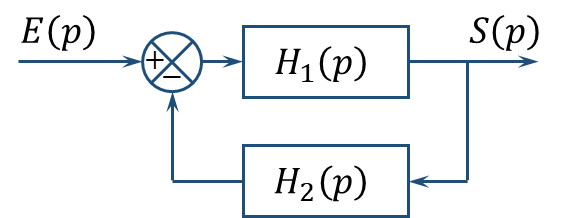
\includegraphics[width=6cm]{fig_01}
\end{center}

	\begin{reponses}	
	\bonne{$\text{FTBO}(p)=H_1(p)H_2(p)$}
	\mauvaise{$\text{FTBO}(p)=H_1(p)$}
	\mauvaise{$\text{FTBO}(p)=\dfrac{H_1(p)}{H_2(p)}$}
	\mauvaise{$\text{FTBO}(p)=\dfrac{H_1(p)}{1+H_1(p)H_2(p)}$}
	\mauvaise{$\text{FTBO}(p)=\dfrac{H_1(p)}{1-H_1(p)H_2(p)}$}
	\end{reponses}

\end{question}\\
}

\element{ftbo}{
\begin{question}{ftbo 02}
Soit le schéma blocs suivant. Donner le FTBO.
\begin{center}
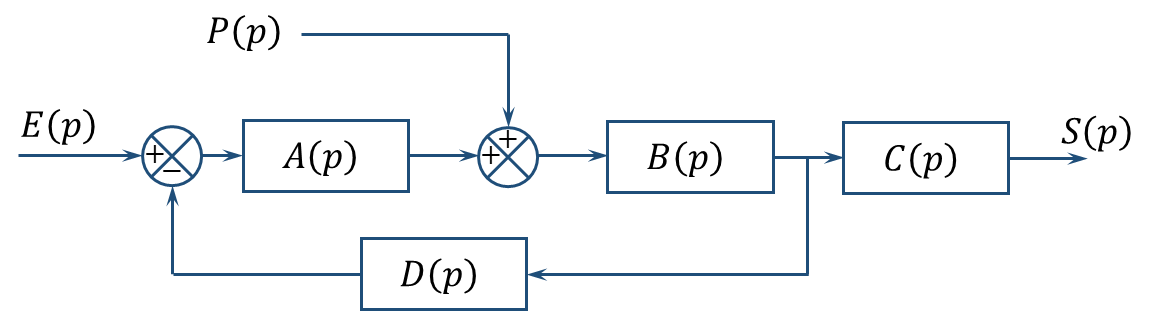
\includegraphics[width=8cm]{fig_02}
\end{center}

	\begin{reponses}	
	\bonne{$\text{FTBO}(p)=A(p)B(p)D(p)$}
	\mauvaise{$\text{FTBO}(p)=A(p)$}
	\mauvaise{$\text{FTBO}(p)=A(p)B(p)C(p)$}
	\mauvaise{$\text{FTBO}(p)=A(p)B(p)C(p)D(p)$}
	\mauvaise{$\text{FTBO}(p)=\dfrac{A(p)B(p)}{1+A(p)B(p)D(p)}$}
	\end{reponses}

\end{question}\\
}


%\element{ftbo}{
%\begin{question}{ftbo 03}
%Soit le schéma blocs suivant. Donner le FTBO.
%\begin{center}
%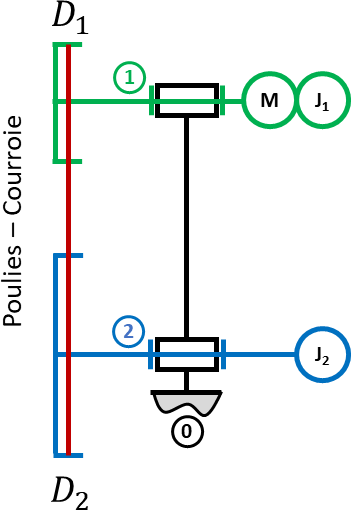
\includegraphics[width=6cm]{fig_03}
%\end{center}
%
%	\begin{reponses}	
%	\bonne{$\text{FTBO}(p)=$}
%	\mauvaise{$\text{FTBO}(p)=$}
%	\mauvaise{$\text{FTBO}(p)=$}
%	\mauvaise{$\text{FTBO}(p)=$}
%	\mauvaise{$\text{FTBO}(p)=$}
%	\end{reponses}
%
%\end{question}\\
%}


\element{ftbo}{
\begin{question}{ftbo 04}
Soit le schéma blocs suivant. Donner le FTBO.
\begin{center}
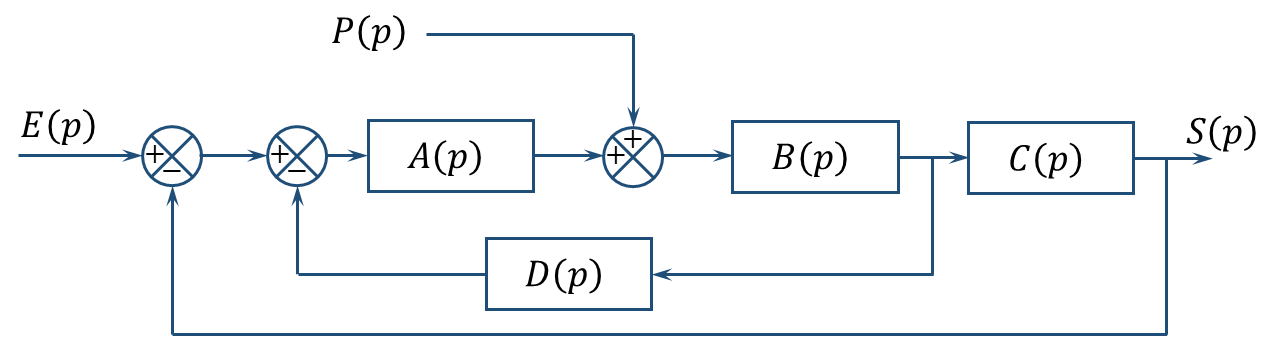
\includegraphics[width=8cm]{fig_04}
\end{center}

	\begin{reponses}	
	\bonne{$\text{FTBO}(p)=\dfrac{A(p)B(p)C(p)}{1+A(p)B(p)D(p)}$}
	\mauvaise{$\text{FTBO}(p)=A(p)B(p)$}
	\mauvaise{$\text{FTBO}(p)=A(p)B(p)C(p)D(p)$}
	\mauvaise{$\text{FTBO}(p)=A(p)B(p)C(p)$}
	\mauvaise{$\text{FTBO}(p)=B(p)C(p)$}
	\end{reponses}

\end{question}\\
}


\element{ftbo}{
\begin{question}{ftbo 05}
Soit le schéma blocs suivant. Donner le FTBO.
\begin{center}
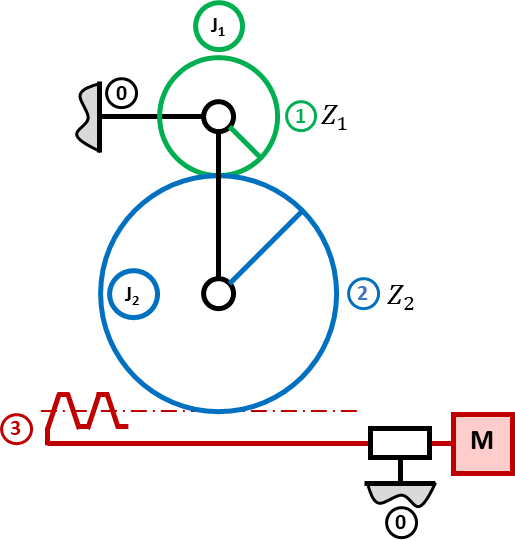
\includegraphics[width=8cm]{fig_05}
\end{center}

	\begin{reponses}	
	\bonne{$\text{FTBO}(p)=\dfrac{A(p)B(p)D(p)}{1+B(p)C(p)}$}
	\mauvaise{$\text{FTBO}(p)=A(p)B(p)C(p)D(p)$}
	\mauvaise{$\text{FTBO}(p)=A(p)B(p)C(p)$}
	\mauvaise{$\text{FTBO}(p)=B(p)C(p)$}
	\mauvaise{$\text{FTBO}(p)=A(p)B(p)D(p)$}
	\end{reponses}

\end{question}\\
}


\element{ftbo}{
\begin{question}{ftbo 06}
Soit le schéma blocs suivant. Donner le FTBO.
\begin{center}
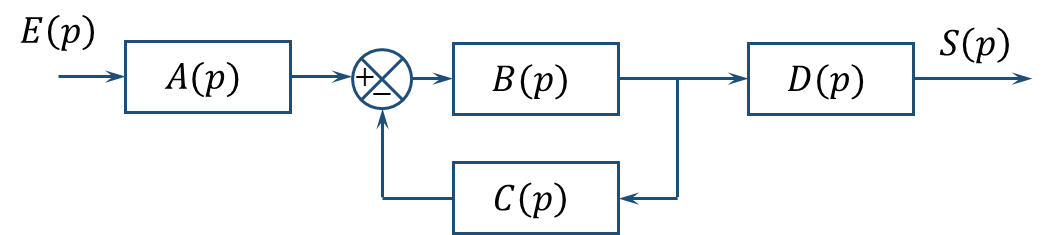
\includegraphics[width=8cm]{fig_06}
\end{center}

	\begin{reponses}	
	\bonne{$\text{FTBO}(p)=B(p)C(p)$}
	\mauvaise{$\text{FTBO}(p)=A(p)B(p)C(p)$}
	\mauvaise{$\text{FTBO}(p)=A(p)B(p)C(p)D(p)$}
	\mauvaise{$\text{FTBO}(p)=\dfrac{A(p)B(p)D(p)}{1+B(p)C(p)}$}
	\mauvaise{$\text{FTBO}(p)=A(p)B(p)D(p)$}
	\end{reponses}

\end{question}\\
}


\element{ftbo}{
\begin{question}{ftbo 07}
Soit le schéma blocs suivant. Donner le FTBO.

\begin{center}
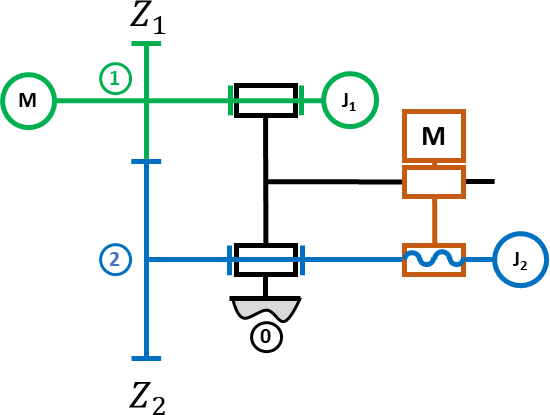
\includegraphics[width=8cm]{fig_07}
\end{center}

	\begin{reponses}	
	\bonne{$\text{FTBO}(p)=\dfrac{A(p)B(p)D(p)}{1+B(p)C(p)D(p)}$}
	\mauvaise{$\text{FTBO}(p)=A(p)B(p)D(p)$}
	\mauvaise{$\text{FTBO}(p)=A(p)B(p)C(p)D(p)$}
	\mauvaise{$\text{FTBO}(p)=\dfrac{A(p)B(p)C(p)}{1+A(p)B(p)D(p)}$}
	\mauvaise{$\text{FTBO}(p)=\dfrac{A(p)B(p)C(p)}{1+B(p)C(p)F(p)}$}
	\end{reponses}

\end{question}\\
}


\element{ftbo}{
\begin{question}{ftbo 08}
Soit le schéma blocs suivant. Donner le FTBO.
\begin{center}
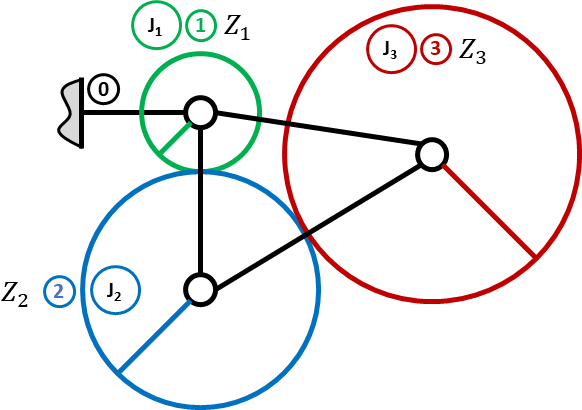
\includegraphics[width=8cm]{fig_08}
\end{center}

	\begin{reponses}	
	\bonne{$\text{FTBO}(p)=B(p)D(p)\dfrac{A(p)-F(p)}{1+B(p)D(p)F(p)}$}
	\mauvaise{$\text{FTBO}(p)=A(p)B(p)D(p)$}
	\mauvaise{$\text{FTBO}(p)=B(p)C(p)$}
	\mauvaise{$\text{FTBO}(p)=A(p)B(p)C(p)$}
	\mauvaise{$\text{FTBO}(p)=\dfrac{A(p)B(p)C(p)}{1+A(p)B(p)D(p)}$}
	\end{reponses}

\end{question}\\
}


\element{ftbo}{
\begin{question}{ftbo 09}
Soit le schéma blocs suivant. Donner le FTBO.
\begin{center}
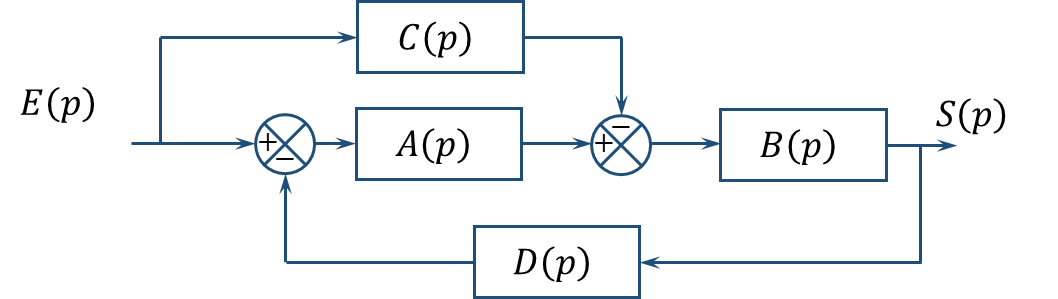
\includegraphics[width=8cm]{fig_09}
\end{center}

	\begin{reponses}	
	\bonne{$\text{FTBO}(p)=B(p)D(p)\dfrac{A(p)-C(p)}{1+B(p)D(p)C(p)}$}
	\mauvaise{$\text{FTBO}(p)=A(p)B(p)D(p)$}
	\mauvaise{$\text{FTBO}(p)=\left(A(p)-C(p)\right)B(p)D(p)$}
	\mauvaise{$\text{FTBO}(p)=A(p)B(p)C(p)$}
	\mauvaise{$\text{FTBO}(p)=\dfrac{A(p)-C(p)}{1+A(p)B(p)D(p)}$}
	\end{reponses}

\end{question}\\
}
